\section{Semantic Location}
\label{sec:sem}

Aside from geometric locations, location semantics are usually more desired by applications.
Imaging a occupancy-driven HVAC controlling system, it is more preferable to locate a person 
at the other corner of the same room she is in, than a nearer point in the adjacent room. Also,
Knowing a person is using a coffee machine or microwave is more interesting than in front of which 
one she is standing. Generally speaking, activity are heavily inter-weaved with localization.
In this section, we propose to use sound to extend the ability to determine transitions of rooms 
of user, as well as sound-based activity recognitions.


\subsection{Environment Transition Detection}
\begin{figure}[H]
\centering
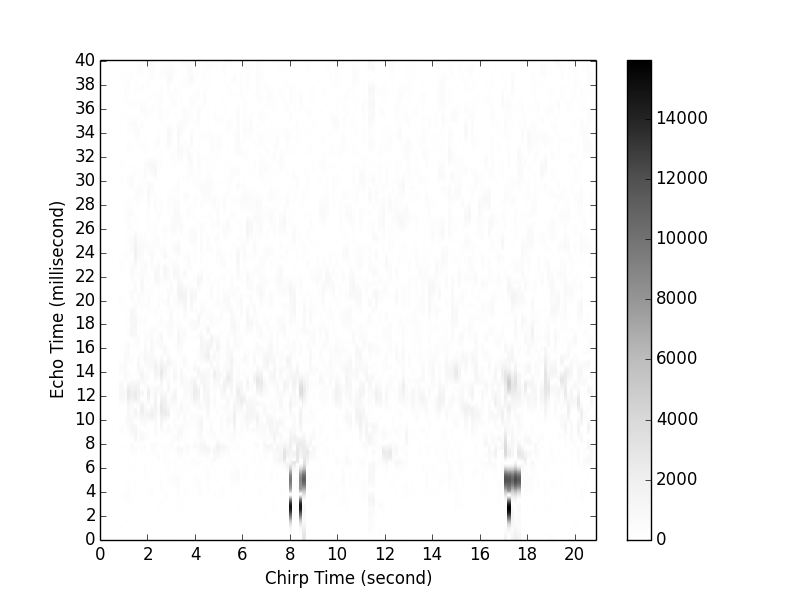
\includegraphics[width=0.45\textwidth]{./fig/transition.png}
\caption{Door Event}
\end{figure}


Rooms mostly come with physical walls in between, particularly when there is demand for 
room-level applications or services, such as room temperature or lighting control. Inferring and 
detecting room transition should be an essential functionality in indoor localization service.
Sound echo is ideal to detect the user going though a wall, which will cause a sudden environment 
change and also acoustic echo pattern change.


Drummer enables continuous environment probing when accelerometer data shows the person is moving.
 


The pattern of 
echoes will have a sudden change when walking through a door or corner.



\subsubsection{Spatial Environment Pattern}

ABS, coffee machine, fridge 